\documentclass[10pt,aspectratio=169]{beamer}
\usetheme{Boadilla}
\usecolortheme{dove}

\usepackage{amsmath}
\usepackage{booktabs}
\usepackage{graphicx}
\usepackage{array}

\graphicspath{{../figures/}}
\setbeamertemplate{navigation symbols}{}
\setbeamertemplate{headline}{}
\setbeamercolor{titlelike}{parent=structure,bg=gray!10}
\setbeamercolor{item}{fg=gray!80}
\setbeamercolor{block title}{bg=gray!20,fg=black}
\setbeamercolor{block body}{bg=gray!5,fg=black}
\setbeamercolor{alertblock title}{bg=red!16,fg=black}
\setbeamercolor{alertblock body}{bg=red!4,fg=black}
\setlength{\parskip}{0pt}
\setbeamertemplate{itemize/enumerate body begin}{\vspace{-0.15em}}
\setbeamertemplate{itemize/enumerate subbody begin}{\vspace{-0.15em}}

\title[Path-dependent technique choice]{Path-Dependent Technique Choice and the Lumpiness of the Red Path}
\subtitle{S90 robustness addendum to CPR preliminary results v6}
\author{Dissertation Chapter 2}
\date{July 2026}

\setbeamertemplate{footline}{%
  \leavevmode%
  \hbox{%
  \begin{beamercolorbox}[wd=.82\paperwidth,ht=2.4ex,dp=1.1ex,leftskip=1em]{author in head/foot}%
    \insertshorttitle\hfill S90 diagnostic: NFC output and NFC capital fixed
  \end{beamercolorbox}%
  \begin{beamercolorbox}[wd=.18\paperwidth,ht=2.4ex,dp=1.1ex,center]{date in head/foot}%
    \insertframenumber/6
  \end{beamercolorbox}}%
}

\begin{document}

% 1
\begin{frame}{1. The red path is not structural $\theta_t$}
  \begin{columns}[T,onlytextwidth]
    \begin{column}{0.57\textwidth}
      \begin{alertblock}{Object correction}
        The red line in v6 is an observed-direction ratio:
        \[
          \vartheta^{path}_{d,t}
          =\frac{\theta g_t^{NRC}+
          (\psi+\lambda\widetilde d_t)(g_t^{ME}-g_t^{NRC})}
          {g_t^{cap}}.
        \]
        It changes when the annual direction of accumulation or its denominator changes.
      \end{alertblock}
      \begin{block}{Structural objects}
        \vspace{-0.7em}
        \[
          \theta^{scale}=\theta,
          \qquad
          \theta^{\tau}_{d,t}=\psi+\lambda\widetilde d_t.
        \]
        These are the equilibrium scale and technique elasticities. Neither equals
        $g_t^p/g_t^{cap}$.
      \end{block}
    \end{column}
    \begin{column}{0.40\textwidth}
      \begin{block}{Coefficient audit}
        \small
        The S34 interaction was orthogonalized over the full panel. Using that same
        projection, primitive and orthogonalized fitted values agree to
        $3.6\times10^{-15}$; manual RDOLS agrees to $5.3\times10^{-15}$.
      \end{block}
      \begin{itemize}\small
        \item Back-transformation reproduces the raw S35 coefficients to rounding precision.
        \item Correcting the coefficients does not remove the lumpy ratio: its roughness remains 79.0\% of the code-as-written path.
        \item v6 should rename the red line before giving it an economic interpretation.
      \end{itemize}
    \end{column}
  \end{columns}
\end{frame}

% 2
\begin{frame}{2. Exact decomposition: the wage term is not the source of the spikes}
  \vspace{-0.4em}
  \begin{columns}[T,onlytextwidth]
    \begin{column}{0.57\textwidth}
      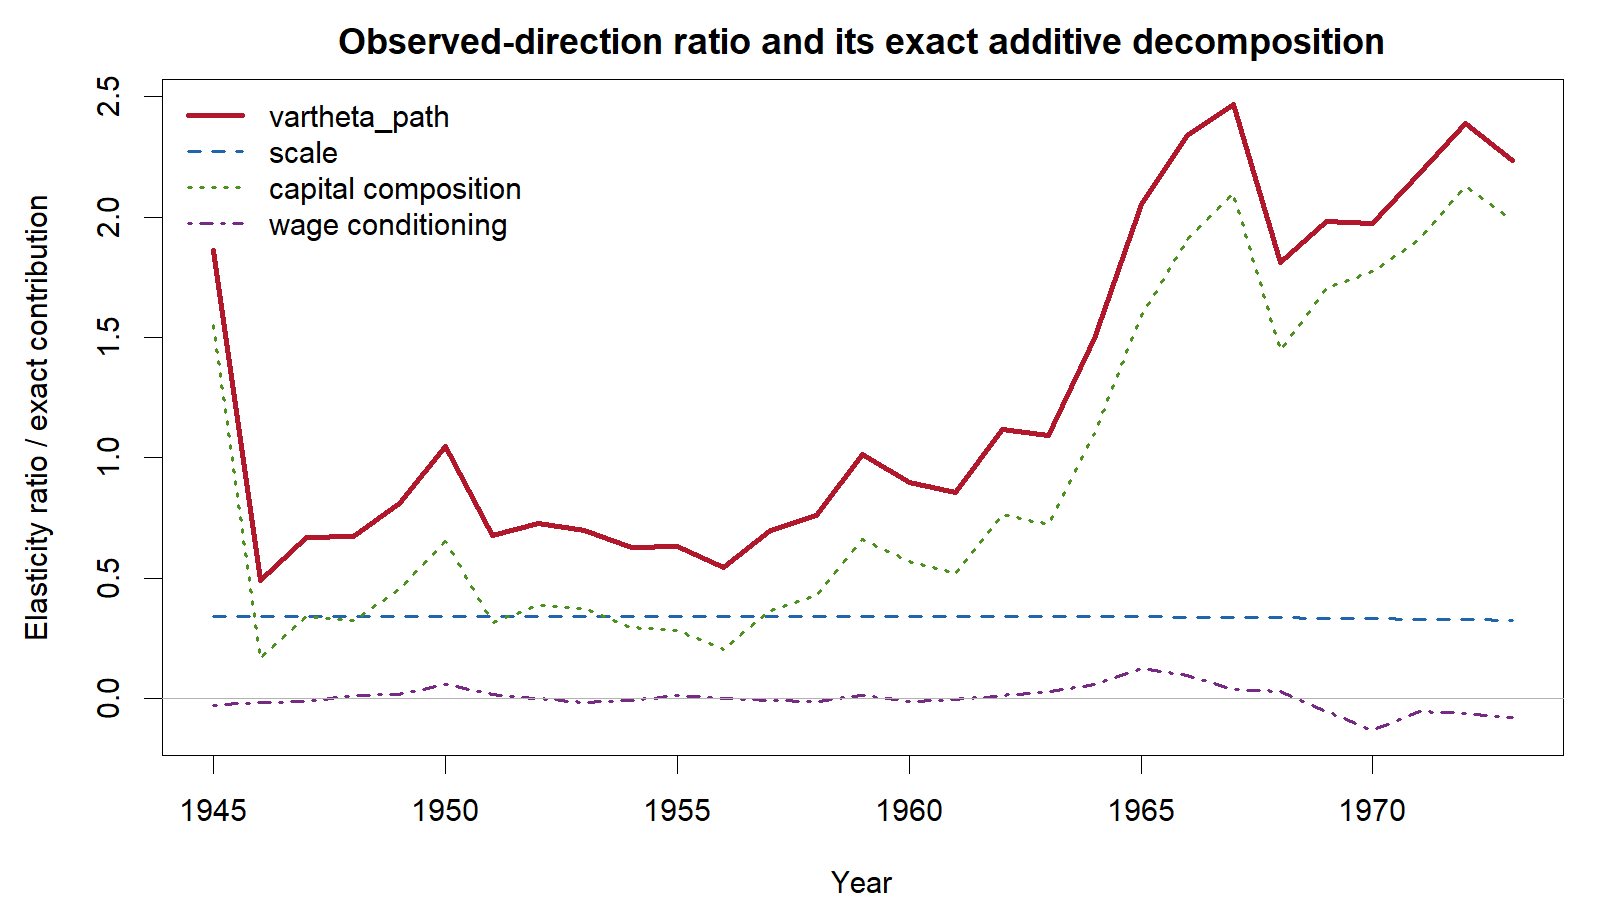
\includegraphics[width=\linewidth]{F01_original_lumpiness_decomposition.png}
    \end{column}
    \begin{column}{0.41\textwidth}
      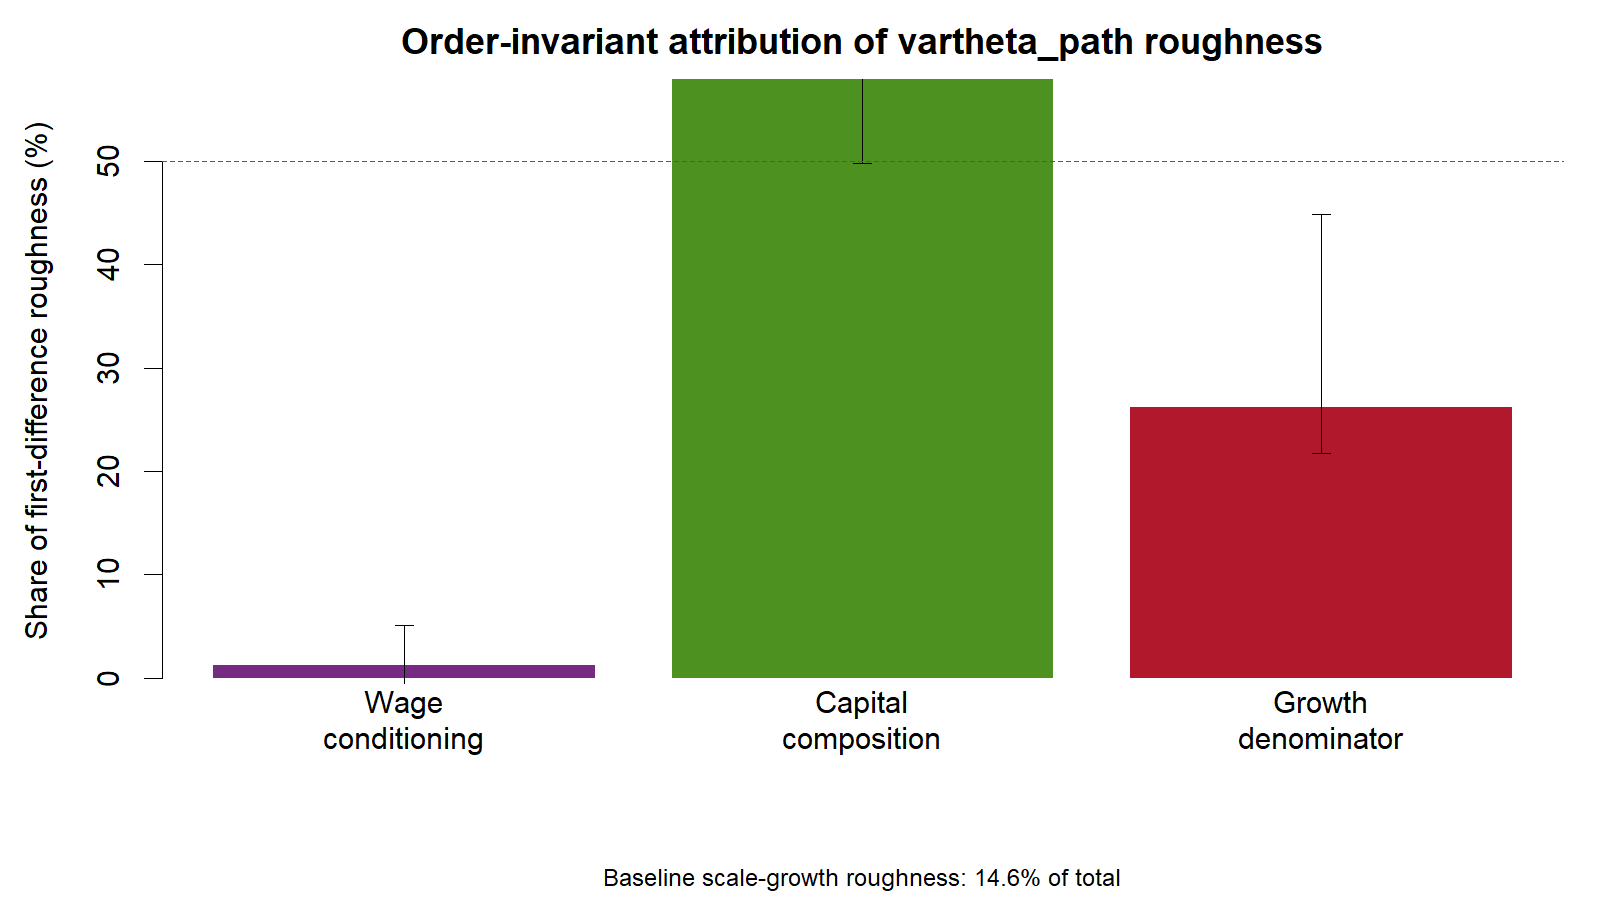
\includegraphics[width=\linewidth]{F05_shapley_attribution.png}
    \end{column}
  \end{columns}
  \vspace{-0.45em}
  \begin{columns}[T,onlytextwidth]
    \begin{column}{0.57\textwidth}
      \scriptsize
      \[
        \vartheta^{path}_{d,t}=C_t^{scale}+C_t^{composition}+C_{d,t}^{distribution},
        \qquad \max|\text{identity error}|=8.9\times10^{-16}.
      \]
    \end{column}
    \begin{column}{0.41\textwidth}
      \scriptsize
      Point Shapley shares: composition 58.0\%, denominator 26.2\%, wage conditioning 1.2\%; baseline structures growth 14.6\%.
      The composition interval is 49.8--67.6\%, so point dominance is not bootstrap-stable.
    \end{column}
  \end{columns}
\end{frame}

% 3
\begin{frame}{3. Wage pressure can cross the productive-capacity boundary}
  \begin{block}{Boundary kept fixed in every run}
    \centering
    $y_t=\log Y_t^{NFC}$, \quad $k_t^{ME}=\log K_t^{ME}$, \quad
    $k_t^{NRC}=\log K_t^{NRC}$, \quad $\tau_t=k_t^{ME}-k_t^{NRC}$.
  \end{block}
  \vspace{-0.2em}
  \begin{table}
    \centering
    \small
    \begin{tabular}{@{}llll@{}}
      \toprule
      \textbf{State} & \textbf{Accounting boundary} & \textbf{Basis} & \textbf{Role} \\
      \midrule
      \texttt{NFC\_GVA}  & whole nonfinancial corporate sector & GVA & main state \\
      \texttt{NFC\_NVA}  & whole nonfinancial corporate sector & NVA & authorized robustness \\
      \texttt{CORP\_GVA} & all corporations & GVA & comparison only \\
      \texttt{CORP\_NVA} & all corporations & NVA & comparison only \\
      \bottomrule
    \end{tabular}
  \end{table}
  \begin{columns}[T,onlytextwidth]
    \begin{column}{0.49\textwidth}
      \begin{block}{Economic sequence}
        \centering
        wage-pressure boundary $\rightarrow$ choice of technique
        $\rightarrow$ NFC capacity building
      \end{block}
    \end{column}
    \begin{column}{0.49\textwidth}
      \begin{alertblock}{Identification limit}
        \small
        Fordist NFC/corporate correlations are 0.998 on both bases. Agreement establishes institutional robustness; it cannot identify a unique bargaining boundary. The GVA alias is exact and is not re-estimated.
      \end{alertblock}
    \end{column}
  \end{columns}
\end{frame}

% 4
\begin{frame}{4. Memory enters technique choice, not the output boundary}
  \begin{columns}[T,onlytextwidth]
    \begin{column}{0.49\textwidth}
      \begin{block}{M0--M1: current state and finite memory}
        \small
        \[
        y_t=\alpha+\theta\widetilde k_t^{NRC}+\psi\widetilde\tau_t
        +\phi\widetilde d_t+\lambda(\widetilde\tau_t\widetilde d_t)+\varepsilon_t,
        \]
        \[
        m_{d,t}^{(h)}=h^{-1}\sum_{j=1}^{h}d_{t-j},\qquad h\in\{3,5\}.
        \]
      \end{block}
      \begin{block}{M2: embodied accumulation}
        \small
        \[
        Q_{\tau,d,t}^{(h)}=\sum_{s\le t}
        (m_{d,s}^{(h)}-\bar m_{d,w}^{(h)})\Delta\tau_s.
        \]
        Wage pressure conditions newly installed technique; it does not revalue the existing stock.
      \end{block}
    \end{column}
    \begin{column}{0.49\textwidth}
      \begin{block}{M3: estimated adaptive memory}
        \small
        \[
          s_{d,t}(\rho)=\rho s_{d,t-1}+(1-\rho)d_{t-1},
          \qquad 0\leq\rho<1,
        \]
        \[
          Q_{\tau,d,t}^{(\rho)}=\sum_{s\le t}
          (s_{d,s}(\rho)-\bar s_{d,w}(\rho))\Delta\tau_s.
        \]
        $\rho$ is profiled on $0.00,0.01,\ldots,0.98$ by Restricted-DOLS BIC.
      \end{block}
      \begin{alertblock}{Estimator discipline}
        \small
        Main correction: manual intercept-only RDOLS LL11. Dynamic terms are restricted to differences of $k^{NRC}$, $\tau$, and the relevant wage state. LL00/LL22 are sensitivities; FM-OLS/IM-OLS are frozen v6 audits only.
      \end{alertblock}
    \end{column}
  \end{columns}
\end{frame}

% 5
\begin{frame}{5. The estimated state is persistent; the main boundary is grid-censored}
  \vspace{-0.4em}
  \begin{columns}[T,onlytextwidth]
    \begin{column}{0.52\textwidth}
      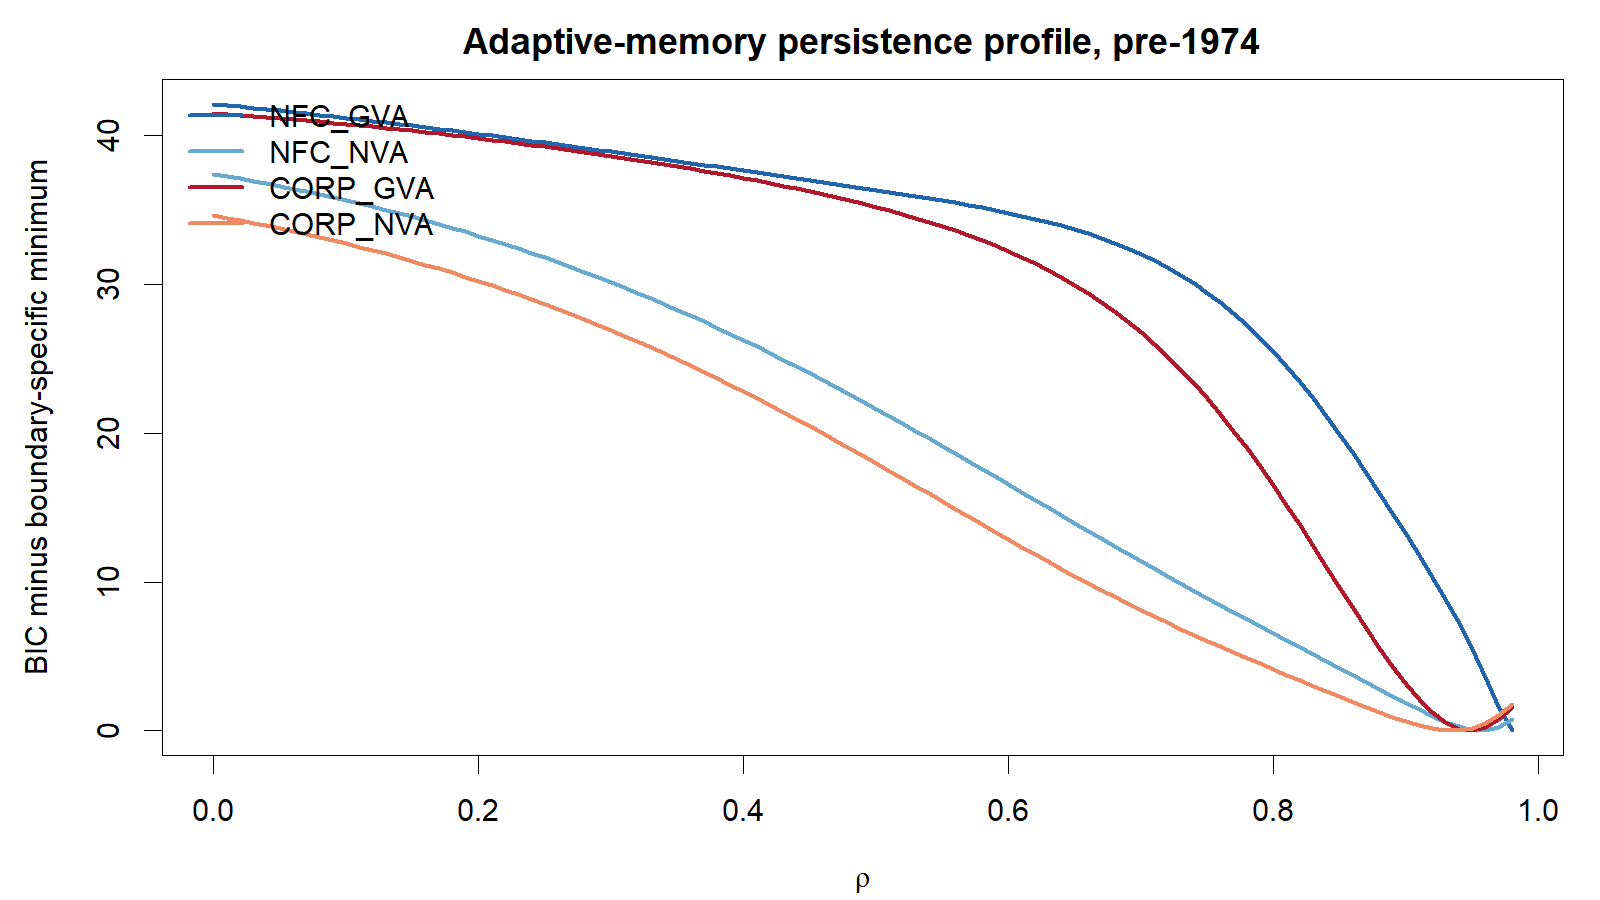
\includegraphics[width=\linewidth]{F06_persistence_profile.png}
    \end{column}
    \begin{column}{0.46\textwidth}
      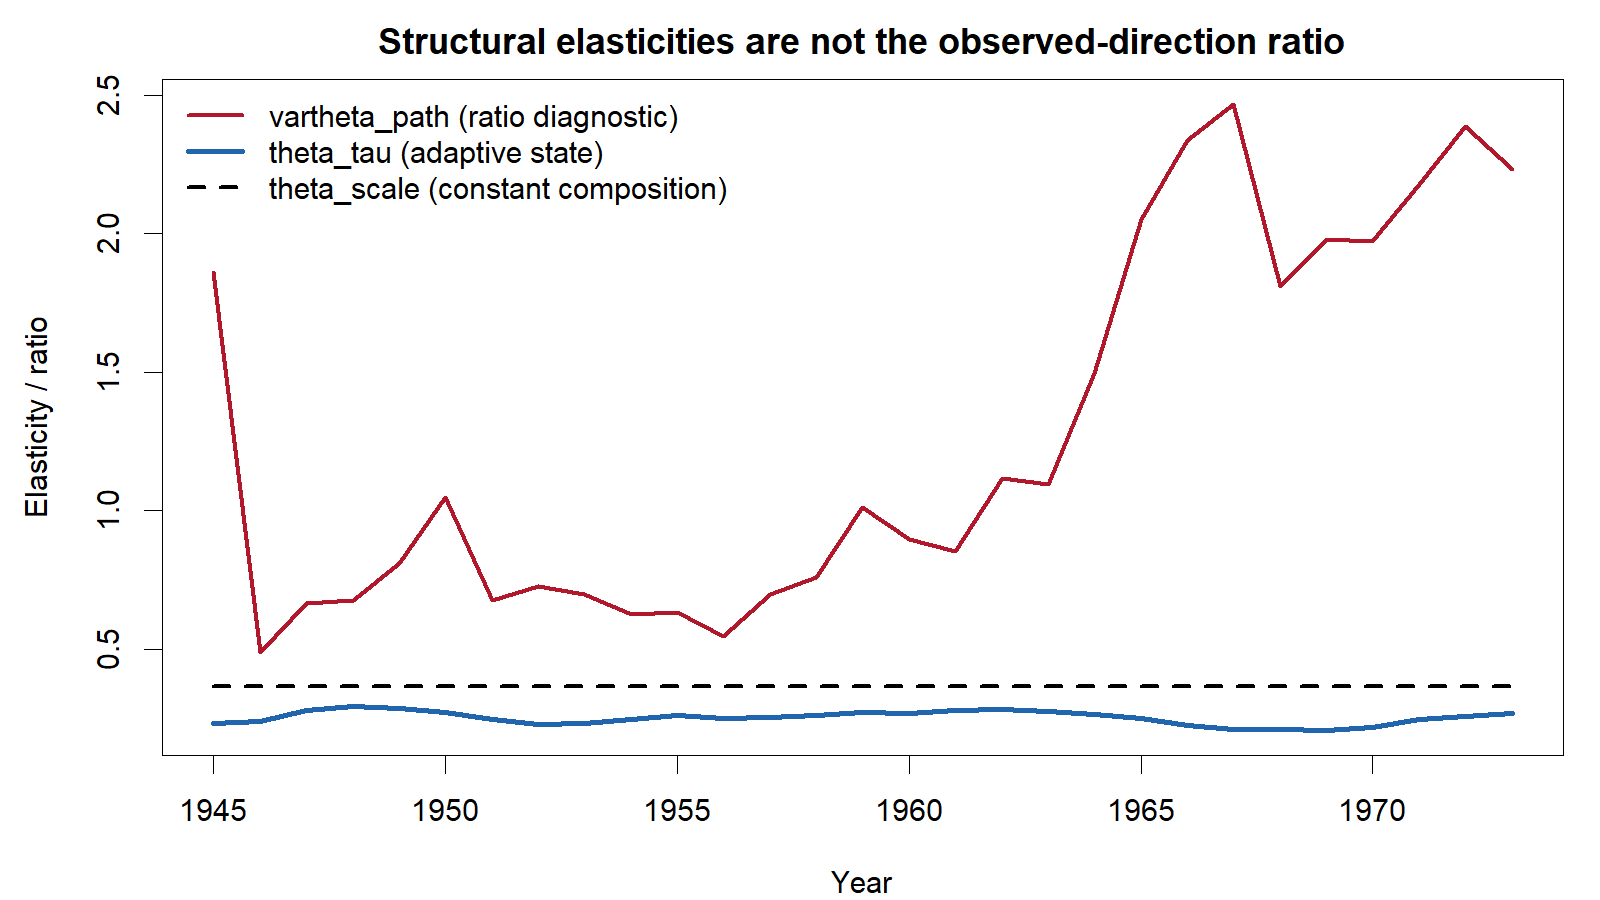
\includegraphics[width=\linewidth]{F02_structural_vs_directional.png}
    \end{column}
  \end{columns}
  \vspace{-0.4em}
  \begin{columns}[T,onlytextwidth]
    \begin{column}{0.52\textwidth}
      \scriptsize
      \begin{tabular}{@{}lccc@{}}
        \toprule
        \textbf{State} & $\hat\rho$ & \textbf{95\% block CI} & \textbf{half-life} \\
        \midrule
        NFC--GVA  & 0.98 & 0.92--0.98 & $\geq 34.3$ y \\
        NFC--NVA  & 0.96 & 0.77--0.98 & 17.0 y \\
        CORP--GVA & 0.95 & 0.86--0.98 & 13.5 y \\
        CORP--NVA & 0.94 & 0.74--0.98 & 11.2 y \\
        \bottomrule
      \end{tabular}
    \end{column}
    \begin{column}{0.46\textwidth}
      \scriptsize
      M2-H3 and M3 pass the generated-path, rank, sample, and residual gates for both NFC definitions; the M2 interaction remains negative under H5. Yet NFC--GVA selects the upper grid boundary, so its half-life is a lower bound and persistence is classified as weak-or-boundary under the prespecified rule.
    \end{column}
  \end{columns}
\end{frame}

% 6
\begin{frame}{6. Verdict and implication for the v6 presentation}
  \begin{columns}[T,onlytextwidth]
    \begin{column}{0.48\textwidth}
      \begin{block}{What the evidence establishes}
        \small
        \begin{itemize}
          \item The red line is a realized-direction ratio, not an equilibrium parameter.
          \item Wage conditioning contributes only 1.2\% of its first-difference roughness.
          \item Unbalanced ME/NRC growth is the point-dominant source (58.0\%); denominator variation contributes another 26.2\%.
          \item The 1945--46 observations account for 54.7\% of attributed roughness, making the ratio data-sensitive under the prespecified rule.
        \end{itemize}
      \end{block}
    \end{column}
    \begin{column}{0.49\textwidth}
      \begin{alertblock}{Adjudication}
        \small
        \textbf{The smoother-equilibrium expectation is not fully supported.}
        Structural $\theta^{scale}$ and $\theta_t^{\tau}$ are materially smoother and both NFC definitions agree, but the main adaptive state is grid-censored and influential capital-growth observations fail the full acceptance rule.
      \end{alertblock}
      \begin{block}{Revise v6 in three places}
        \small
        \begin{enumerate}
          \item Rename the red line ``observed-direction capacity payoff (ratio diagnostic).''
          \item Report $\theta^{scale}$, $\theta_t^{\tau}$, and $g_t^p$ before dividing by $g_t^{cap}$.
          \item Present embodied/adaptive memory as S90 robustness evidence, not as a replacement for the locked chapter specification.
        \end{enumerate}
      \end{block}
    \end{column}
  \end{columns}
\end{frame}

\end{document}
